\section{问题三：滚动预报下的“计划—调整—紧急”模型}
\label{sec:q3}

\subsection{模型建立}

问题三在每个预报时刻都可获得“未来 24 小时整点光伏预报”，因此构成一个
\textbf{滚动时域（MPC）三段决策}问题：0:00 制定全天计划，6:00/12:00/18:00
依据最新预报对\textbf{剩余时段}重新优化并继承当前储电量。

记计划量为 $P^0_t$，调整后量为 $P_t$，定义计划的“超出量”与“调整超出量”
\begin{equation}
S_t=\text{max}\{0,\ P^0_t-P_t\},\qquad X_t=\text{max}\{0,\ P_t-P^0_t\},
\label{eq:SX}
\end{equation}
则逐时段计价（按题面规则）为
\begin{equation}
c_t=\underbrace{p_t\text{min}(P^0_t,P_t)}_{\text{共同部分按基准价}}
+\underbrace{0.5\,p_t S_t}_{\text{违约电价 50\%}}
+\underbrace{1.5\,p_t X_t}_{\text{超出部分 1.5 倍}} .
\label{eq:q3price}
\end{equation}
由于 $S_t,X_t$ 只需满足 $P_t+S_t-X_t=P^0_t$ 且非负，式 \eqref{eq:q3price} 为分段线性函数，
可用两个非负辅助变量精确线性化，因此整个过程仍是 LP。

\textbf{（1）0:00 计划}：以第 \ref{sec:q2} 节的升级预测模型（负荷分类组合、光伏岭回归堆叠）
与报童裕度 $q^*=0.7$ 为输入求解式 \eqref{eq:obj}--\eqref{eq:c5}，得到 $P^0_t,C^0_t,D^0_t$。

\textbf{（2）$t_0$ 时刻的滚动调整}：以已锁定计划 $P^0_{t\ge t_0}$ 为基准，
对剩余时段求解\textbf{增量优化}：
\begin{align}
\text{min}\quad & \sum_{t\ge t_0}\Big(-0.5\,p_tS_t+1.5\,p_tX_t\Big)-vE_{145}
\label{eq:adj_obj}\\
\text{s.t.}\quad & \widehat{PV}^{t_0}_t+D_t-C_t+P_t\ \ge\ \tilde N^{t_0}_t,\qquad
\tilde N^{t_0}_t=\hat L^{t_0}_t-\widehat{PV}^{t_0}_t+b^{t_0}_t, && t\ge t_0 \label{eq:adj_bal}\\
& E_{t+1}=E_t+\eta_cC_t-\frac{D_t}{\eta_d},\quad 1200\le E_t\le10800, && t\ge t_0 \label{eq:adj_soc}\\
& P_t+S_t-X_t=P^0_t,\quad S_t,X_t\ge0,\quad 0\le C_t,D_t\le\bar C,\quad P_t\ge0. && \label{eq:adj_link}
\end{align}
其中 $\widehat{PV}^{t_0}_t$ 取 $t_0$ 时刻最新发布的预报（整点功率点线性插值到 10 分钟）。
\textbf{关键细节}：调整之后重新面对的是“剩余时段的不确定性”，因此必须
\textbf{按新预报的口径重设报童裕度}
\begin{equation}
b^{t_0}_t=\mathrm{Quantile}_{q}\Big\{\big[(L-PV)-( \hat L^{t_0}-\widehat{PV}^{t_0})\big]_{\tau,t}\Big\}_{\tau\in\text{近30天}},
\label{eq:adjbuffer}
\end{equation}
即用“该时刻预报”的历史残差经验分位作为裕度。若沿用 0:00 的裕度（或干脆不带裕度），
调整后的计划将没有任何安全余量，全年费用反而升到 14\,704\,403 元
（比不调整贵 104.9 万元）——这说明\textbf{“调整”本身也是不确定性下的决策，必须同样保守}。

\textbf{（3）日内执行}：与问题二一致，按 0:00/调整时定下的\textbf{平衡响应规则}
（式 \eqref{eq:clip}--\eqref{eq:socrec}）执行：先动用计划充放电的可调空间、
再动用储能存量，兜不住的缺口才按 $5p_t$ 紧急购电，富余则弃光。
调整后当日总费用为
\begin{equation}
\text{Cost}_d=\sum_t p_tP^0_t+\sum_t\Big(-0.5p_tS_t+1.5p_tX_t\Big)+\sum_t 5p_tE^{\text{急}}_t .
\label{eq:q3cost}
\end{equation}

\subsection{结果：是否需要引入其他时刻的预报}

\begin{table}[htbp]
\centering
\caption{问题三：不同滚动方案全年（2.1--12.31）费用对照（单位：元）}
\label{tab:q3cmp}
\small
\begin{tabular}{@{}lcccc@{}}
\toprule
方案 & 计划购电费 & 调整相关费用 & 紧急购电费 & 总费用 \\
\midrule
仅用 0:00 计划（不做调整） & 12\,866\,999 & 0 & 788\,836 & 13\,655\,835 \\
$+6{:}00$ 调整 & 12\,866\,908 & 281\,105 & 691\,758 & 13\,839\,771 \\
\textbf{$+12{:}00$ 调整（采用）} & \textbf{12\,866\,905} & \textbf{106\,920} & \textbf{603\,066} & \textbf{13\,576\,891} \\
$+18{:}00$ 调整 & 12\,867\,059 & 11\,950 & 789\,181 & 13\,668\,190 \\
$+6{:}00$、$+12{:}00$ 调整 & 12\,866\,866 & 204\,664 & 515\,441 & 13\,586\,971 \\
$+12{:}00$、$+18{:}00$ 调整 & 12\,866\,848 & 112\,648 & 596\,183 & 13\,575\,679 \\
全滚动（6/12/18） & 12\,866\,817 & 209\,428 & 507\,355 & 13\,583\,600 \\
完全信息下界（天眼链式） & 12\,286\,531 & 0 & 0 & 12\,286\,531 \\
\bottomrule
\end{tabular}
\end{table}

\textbf{各时刻的边际价值}（以“不做调整”为基准，\cref{tab:q3cmp}）：
\begin{equation}
\Delta_{6:00}=-18.39\ \text{万元},\qquad
\Delta_{12:00}=+7.89\ \text{万元},\qquad
\Delta_{18:00}=-1.24\ \text{万元},\qquad
\Delta_{\text{全滚动}}=+7.22\ \text{万元}.
\label{eq:marginal}
\end{equation}

因此对题面所问“是否需要引入其他时刻的预报制定调整策略”，本文的结论是：

\begin{enumerate}[label=(\arabic*), leftmargin=2.4em, itemsep=1pt]
\item \textbf{需要，而且只需 12:00 一次}。12:00 的调整把计划购电量按最新预报重新分配
（下调 305\,156 kWh、上调 522\,468 kWh 中的一部分），紧急购电费由 78.9 万元降到 60.3 万元，
净节约 \textbf{7.89 万元（0.58\%）}；而 $+12{:}00$ 与 $+18{:}00$ 组合只再多省 0.01\%（1\,212 元），
属于数值噪声。
\item \textbf{6:00 与 18:00 的预报不值得引入}。6:00 单独调整反而贵 18.39 万元：
此时“最新预报”相对 0:00 依据并无实质改进（剩余时段光伏 MAE 180.1 kW vs 我们 0:00 依据的 177.9 kW），
却要付 28.1 万元偏差费；18:00 之后光伏已接近零，新预报几乎不含信息（我们 0:00 依据的
剩余时段 MAE 仅 6.4 kW，反而优于该时刻预报的 15.8 kW），调整只值 $-1.24$ 万元。
\item \textbf{调整的价值来自“更好的预报”，不是“更多的时刻”}：12:00 的预报在剩余时段
确实更准（光伏 113.4 kW vs 140.1 kW；\textbf{净需求 206.1 kW vs 234.6 kW}，
而净需求才是计划 LP 的真正输入），因此值得付一次偏差费；这类判断与第 \ref{sec:compare} 节的
敏感性分析一致：偏差计价（0.5/1.5 倍）是调整的“手续费”，
\textbf{只有当新预报带来的紧急购电节省超过手续费时，调整才是划算的}。
\end{enumerate}

\begin{figure}[htbp]
\centering
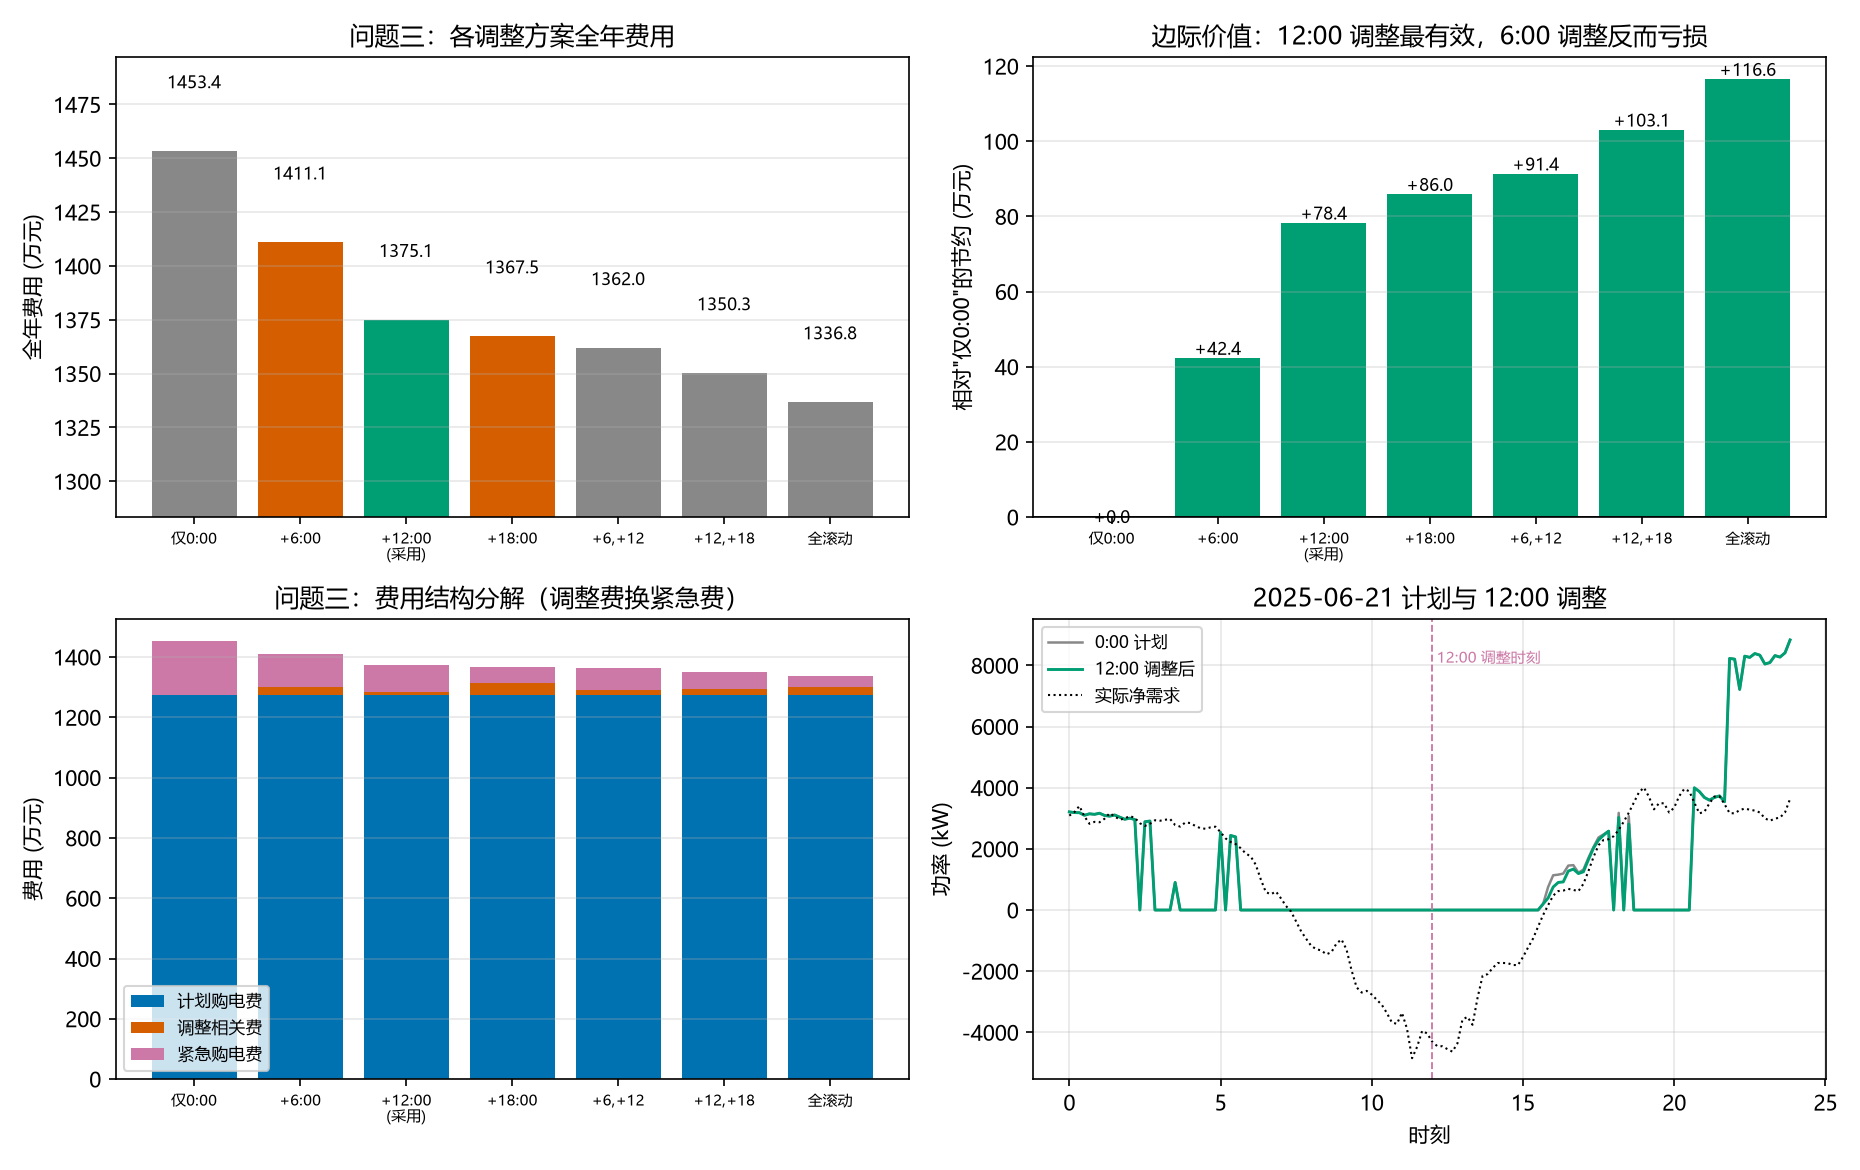
\includegraphics[width=0.95\textwidth]{figures/fig_q3_rolling.png}
\caption{问题三：各调整方案全年费用（左上）、调整的边际价值（右上）、费用结构分解（左下）、
2025-06-21 计划与 12:00 调整（右下）}
\label{fig:q3}
\end{figure}

\subsection{指定日期结果（表 1、表 2、表 3 格式）}

\begin{table}[htbp]
\centering
\caption{问题三：指定日期关键时段计划购电量与全天购电量、购电费（表 1 格式，kWh/元）}
\label{tab:q3t1}
\scriptsize
\begin{tabular}{@{}lcccc@{}}
\toprule
时间段 & 2025-03-20 & 2025-06-21 & 2025-09-23 & 2025-12-21 \\
\midrule
10:00--10:10 & 0.00 & 0.00 & 0.00 & 0.00 \\
12:00--12:10 & 572.73 & 0.00 & 417.97 & 970.56 \\
14:00--14:10 & 0.00 & 0.00 & 0.00 & 0.00 \\
16:00--16:10 & 564.40 & 210.12 & 565.82 & 847.33 \\
18:00--18:10 & 702.62 & 0.00 & 775.60 & 716.85 \\
20:00--20:10 & 0.00 & 0.00 & 0.00 & 0.00 \\
\midrule
全天购电量 & 69\,247.84 & 37\,122.93 & 68\,473.30 & 97\,053.33 \\
全天购电费 & 41\,846.37 & 21\,173.98 & 42\,567.28 & 62\,140.33 \\
调整后全天购电量 & 66\,614.94 & 36\,796.67 & 67\,806.68 & 97\,738.36 \\
调整后购电相关费 & 41\,126.78 & 21\,183.30 & 42\,534.46 & 62\,832.29 \\
\bottomrule
\end{tabular}
\end{table}

\begin{table}[htbp]
\centering
\caption{问题三：指定日期最终储能充放电量与 0:00、24:00 储电量（表 2 格式，kWh）}
\label{tab:q3t2}
\scriptsize
\begin{tabular}{@{}lcccccccc@{}}
\toprule
\multirow{2}{*}{时间段} & \multicolumn{2}{c}{2025-03-20} & \multicolumn{2}{c}{2025-06-21} &
\multicolumn{2}{c}{2025-09-23} & \multicolumn{2}{c}{2025-12-21} \\
\cmidrule(lr){2-3}\cmidrule(lr){4-5}\cmidrule(lr){6-7}\cmidrule(lr){8-9}
& 充电 & 放电 & 充电 & 放电 & 充电 & 放电 & 充电 & 放电 \\
\midrule
0:00--4:00 & 120.41 & 177.57 & 90.73 & 3628.48 & 112.35 & 58.65 & 72.60 & 100.04 \\
4:00--8:00 & 169.32 & 5935.75 & 389.36 & 4839.09 & 178.05 & 6091.11 & 854.59 & 1456.11 \\
8:00--12:00 & 6028.92 & 2761.36 & 9973.71 & 0.00 & 5607.93 & 1896.62 & 5592.70 & 7159.56 \\
12:00--16:00 & 4298.32 & 311.10 & 0.00 & 0.00 & 4598.44 & 465.74 & 7006.37 & 2240.55 \\
16:00--20:00 & 297.38 & 5789.99 & 185.75 & 5541.23 & 121.80 & 5728.82 & 0.86 & 5829.30 \\
20:00--24:00 & 10\,723.59 & 2550.96 & 9726.06 & 2487.33 & 10\,644.52 & 2973.49 & 10\,666.67 & 2811.39 \\
\midrule
0:00 储电量 & \multicolumn{2}{c}{10\,800.00} & \multicolumn{2}{c}{10\,800.00} &
\multicolumn{2}{c}{10\,746.31} & \multicolumn{2}{c}{10\,800.00} \\
24:00 储电量 & \multicolumn{2}{c}{10\,800.00} & \multicolumn{2}{c}{10\,800.00} &
\multicolumn{2}{c}{10\,755.97} & \multicolumn{2}{c}{10\,800.00} \\
\bottomrule
\end{tabular}
\end{table}

\begin{table}[htbp]
\centering
\caption{问题三：指定日期紧急购电时间段与购电量（表 3 格式，kWh）}
\label{tab:q3t3}
\scriptsize
\begin{tabular}{@{}llll@{}}
\toprule
2025-03-20（合计 441.38） & 2025-06-21 & 2025-09-23（合计 208.36） & 2025-12-21（合计 31.13） \\
\midrule
9:50--10:00\ 16.02 & \multicolumn{1}{c}{无紧急购电} & 20:20--20:40\ 124.27 & 20:30--20:40\ 31.13 \\
20:30--20:40\ 425.36 & & 20:50--21:10\ 81.13 & \\
 & & 21:20--21:30\ 2.96 & \\
\bottomrule
\end{tabular}
\end{table}

对比\cref{tab:q2t3} 与\cref{tab:q3t3} 可见：12:00 调整后 2025-09-23 的紧急购电量由
228.74 kWh 降到 208.36 kWh、2025-12-21 保持 31.13 kWh，而 2025-03-20 由 54.68 kWh
升到 441.38 kWh（12:00 的预报偏乐观，计划量被下调，风险后移）。这与式 \eqref{eq:marginal}
的结论一致：\textbf{调整的收益主要来自“按最新预报重新分配购电时段”的
计划购电费变化与紧急购电费变化之差}，而不是单看某一天的紧急电量。
